\documentclass{article}

\usepackage[final,nonatbib]{nips_2017}

\usepackage[utf8]{inputenc} % allow utf-8 input
\usepackage[T1]{fontenc}    % use 8-bit T1 fonts
\usepackage{hyperref}       % hyperlinks
\usepackage{url}            % simple URL typesetting
\usepackage{booktabs}       % professional-quality tables
\usepackage{amsfonts}       % blackboard math symbols
\usepackage{nicefrac}       % compact symbols for 1/2, etc.
\usepackage{microtype}      % microtypography

\usepackage[backend=biber]{biblatex}
\addbibresource{report.bib}

\usepackage{graphicx}
\graphicspath{ {images/} }

% https://tex.stackexchange.com/questions/376420/include-chinese-characters-into-article-in-xelatex
\usepackage{fontspec}
\newfontfamily\cjkfont{Noto Sans CJK SC}

\usepackage{listings}

\title{Snowbot: An empirical study of building chatbot using seq2seq model with different machine learning framework}

\author{
Pinglei Guo \\
\texttt{piguo@ucsc.edu} \\
\And
Yusi Xiang \\
\texttt{yxiang12@ucsc.edu} \\
\And
Yunzheng Zhang \\
\texttt{yzhan300@ucsc.edu} \\
\And
Weiting Zhan \\
\texttt{wzhan83@ucsc.edu} \\
}

\begin{document}

\maketitle

\begin{abstract}
    Chatbot is a growing topic, we built a open domain generative chatbot using seq2seq model with different machine learning framework (Tensorflow, MXNet).
    Our result show although seq2seq is a successful method in neural machine translation, use it solely on single turn chatbot yield pretty unsatisfactory result.
    Also existing free dialog corpus lacks both quality and quantity.
    Our conclusion it's hard to build a useful open domain generative bot using state of art technology.
\end{abstract}

\section{Introduction}
\label{sec:introduction}

\subsection{Chatbot}
\label{subsec:chatbot}

Chatbot can be generally divided into two types, open domain and close domain.
Former can answer a wide range of questions (though the answer itself could be very general with syntax and semantic error),
latter can solve particular problems from user, and user is not expecting a close domain bot to chat freely as well.
Based on how response is generated, it can be divided to retrieval and generative,
where answer is picked from clustered responses~\cite{kannan2016smart} or generated on the fly.
In theory, open domain chatbot has more potential\footnote{if the domain is really open enough, generate random text might be the best algorithm},
and is harder to build, in practice, most chatbot that gets work done is close domain,
even those that seems to be open domain (Siri, Cortana) are not implemented end to end, heuristic rules, entity recognition, knowledge base,
clustered response are inject into multiple stages in the pipeline to produce good result.

At first (during proposal) we believe a close domain retrieval chatbot is the most easy one in the total four combinations based on a blog post~\cite{wildml},
Then we realize that this is the most easy one in theory but the hardest one in practice, the other corner,
open domain generative is actually easiest because it's end to end, just two RNN is enough.
% And there is no hard metrics for evaluating a open domain chatbot~\cite{liu2016not}.
Thus we decided to build a open domain generative chatbot in the limited time given.

\subsection{Machine Learning Frameworks}
\label{subsec:ml-frameworks}

Machine learning framework is now the competing spot for tech giants (Table~\ref{table:ml-frameworks}), besides they are using ML excessively in their own products,
they want developers to use their framework and run it on their cloud platform, (i.e. Tensorflow on Google Cloud, MXNet on AWS, CNTK on Azure).
Although there were many open source frameworks started by individual and research organizations, most of them are deprecated
in favor of those backed by companies (i.e. Theano vs. Tensorflow)\footnote{\url{https://groups.google.com/forum/\#!msg/theano-users/7Poq8BZutbY/rNCIfvAEAwAJ}}

\begin{table}[h]
    \caption{Popular Machine learning Frameworks}
    \label{table:ml-frameworks}
    \centering
    \begin{tabular}{llll}
        \toprule
        Name & Star & Company & First Release\\
        \midrule
        \href{https://github.com/tensorflow/tensorflow}{Tensorflow} & 81697 & Google & 2015-11-08 \\
        \href{https://github.com/keras-team/keras}{Keras} & 22872 & N/A & 2015-01-13 \\
        \href{https://github.com/BVLC/caffe}{Caffe} & 21739 & N/A & 2014-03-19 \\
        \href{https://github.com/Microsoft/CNTK}{CNTK} & 13366 & Microsoft & 2016-01-22 \\
        \href{https://github.com/apache/incubator-mxnet}{MXNet} & 12392 & Amazon & 2015-12-09 \\
        \href{https://github.com/pytorch/pytorch}{PyTorch} & 10142 & Facebook & 2016-08-31 \\
        \href{https://github.com/torch/torch7}{Torch} & 7537 & N/A & 2015? \\
        \bottomrule
    \end{tabular}
\end{table}

Tensorflow~\cite{abadi2016tensorflow} and MXNet~\cite{chen2015mxnet} are two widely used frameworks, while tensorflow is
mostly declarative, mxnet allows more imperative programming style.
A simple example is in order to debug the value of a matrix in tensorflow you need to write an op using \verb+tf.Print+ and put it inside compute graph,
while in mxnet you can just use \verb+print+ like it's a normal python variable, though in fact it might resides on GPU or other machines.
Declarative style is not very expressive, but make optimization on the framework side easier, mxnet chose to detect patterns
and only optimize critical path to gain flexibility while retain performance.
However, when it comes to most software engineers, the design and low-level API does not matter much,
community support and a wide range of up to date model is more important, and tensorflow is the obvious winner.
For researchers, mxnet might be a better choice, since it has thinner wrapper and stricter requirement.

We chose to use two higher level seq2seq frameworks, sockeye (based on mxnet)\footnote{\url{https://github.com/awslabs/sockeye}}
and OpenNMT-tf\footnote{\url{https://github.com/OpenNMT/OpenNMT-tf}} in the experiments,
we did try to write a naive one based on newer seq2seq API in tensorflow, however since both sockeye and OpenNMT-tf use state of art models
and yield unsatisfactory result, we abandoned it in the middle \footnote{\url{https://github.com/at15/snowbot/pull/23}}.

The rest of the report is organized as following, Section~\ref{sec:model} describes the basic form of the seq2seq model we are using.
Section~\ref{sec:dataset} shows how we process our dataset, and the problem in it.
Implementation detail is listed in section~\ref{sec:implementation}.
Our result is shown in section~\ref{sec:evaluation}.
Section~\ref{sec:conclusion} concludes the report and \textbf{workload distribution}.

\section{Model}
\label{sec:model}

We use seq2seq model, which is widely used in neural machine translation~\cite{sutskever2014sequence}
and can be applied to single turn dialog system (QA) as well.
Its basic structure is two recurrent neural networks (RNN) as shown in figure~\ref{fig:seq2seq}.
The cell used in RNN is LSTM (long term short memory),
so we can learn implicit relation ship between words from data without explicit pre-processing.
seq2seq is one of many variants of RNN + LSTM. Based on the domain and length of input,
RNN + LSTM can be used for sequence classification, text generation, translation, dialog system etc.
as shown in table~\ref{table:RNN+LSTM}

\begin{table}[h]
    \caption{Variants of RNN + LSTM}
    \label{table:RNN+LSTM}
    \centering
    \begin{tabular}{llll}
        \toprule
        Type & Input & Output & Example \\
        \midrule
        seq2one (classification) & sentence & class & Sentiment analysis \\
        seq2seq (text generation) & sentence & same sentence & Shakespeare style text \\
        seq2seq (translation) & language A & language B & NMT A -> B \\
        seq2seq (single turn QA) & question & answer & chatbot \\
        seq2seq (multi turn QA) & conversation context & answer & chatbot \\
        \bottomrule
    \end{tabular}
\end{table}

For many to many in RNN + LSTM (seq2seq), simply swap the input and output data, you get a different application for free
(Table~\ref{table:seq2seq-app}) \footnote{not real data, for demonstration only}.
So we can use neural machine translation framework directly to build our chatbot.

\begin{table}[h]
    \caption{Input and Output of different seq2seq application}
    \label{table:seq2seq-app}
    \centering
    \begin{tabular}{lllll}
        \toprule
        Type & Train input & Train output & Test input & Test output \\
        \midrule
        text generation & You are my foe & You are my foe & You are & my <unk>\\
        translation & {\cjkfont 你好} & Hello & {\cjkfont 吃了么} & Good morning \\
        single turn QA & Any idea & I don't know & How's the weather & I don't know \\
        multi turn QA & Got it?; No; Why? & I don't know & Hi; Hey; What's up? & I don't know \\
        \bottomrule
    \end{tabular}
\end{table}

\begin{figure}[h]
    \centering
    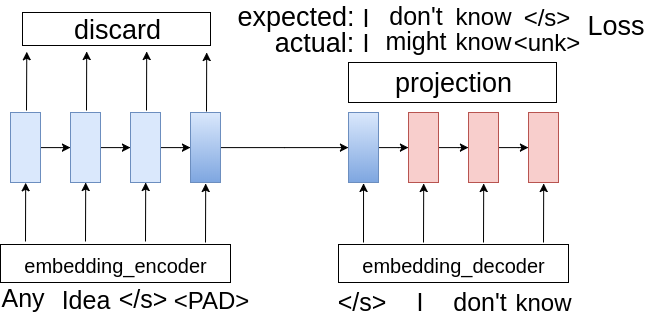
\includegraphics[width=\columnwidth]{seq2seq-simple}
    \caption{Sequence to Sequence model for single turn Dialog}
    \label{fig:seq2seq}
\end{figure}

From figure~\ref{fig:seq2seq} we can see the main idea of seq2seq is to encode input words sequence into a vector,
and decode this vector until reaches max step or EOS (\verb+</s>+).
On the encoder side, the output and hidden state are all discarded except the last hidden state,
which certainly lose some important information, and leads to optimization like attention~\cite{luong2015effective}.

% TODO: add graph

On the decoder side, train and test (infer) is different.
The first word is \verb+<s>+ instead of real word in both case, but in training, the word feed into each step is from
original data while in testing, the word feed into each step is based on the output of previous step.
The output from projection layer (after softmax) is a vector indicating probability of each word in vocabulary.
In training, we calculate loss use cross entropy, note that due to the length of sequences in a mini batch may not be the same,
we use padding (\verb+<PAD>+) to form a matrix and we need to mask those padded part out when calculating loss.
In test, we can pick the word with max probability as word for this step, this is the greedy way,
but we may not pick the overall best sentence if we consider each word independently.
A better way is to use Beam Search, which is keep top-K words in each step, and take the path of top-1 as the final output.

In sockeye and OpenNMT-tf, both attention and beam search are enabled by default, also there can be more than one layer LSTM
or combination of cells (bi-direction), in original NMT paper they say feed input in reverse order increase performance~\cite{sutskever2014sequence},
and with bi-direction, a sentence is feed into encoder in two directions.

\section{Dataset}
\label{sec:dataset}

\subsection{Handling I don't know in Cornell Movie Dialog Corpus}
\label{subsec:idk}

We start with Cornell Movie Dialog Corpus~\cite{data:cornell} because it is used by many publication and blog posts for single turn dialog system.
It contains 83097 conversations, and can be converted to 221282 single turn QA, total file size is 22MB.

However, our first run using sockeye shows \verb+I don't know+ is the most popular response (Table \ref{table:cornell-idk} left),
which leads to a very simple questions. How many \verb+I don't know+ do we have in training data,
does the bot learn to know what it really knows, or there are just too many \verb+I don't know+ in training data.

So we add counting and removing \verb+I don't know+ when processing text.
There are 5114 response is just \verb+I don't know+, which is 2.3\%., excluding those with \verb+I don't know+ as prefix.
Considering the corpus is from movie with varies backgrounds, 2.3\% is a relative high percentile.
After removing I don't know, the responses (Table~\ref{table:cornell-idk} right) become very general questions like \verb+what do you mean+.

\begin{table}[h]
    \caption{Cornell corpus before and after filtering out I don't know}
    \label{table:cornell-idk}
    \centering
\begin{tabular}{p{70mm}|p{70mm}}
  \toprule
  Raw text without processing & After filtering out I don't know \\
  \hline
  Q: hi \newline
A: I don't want to talk to you. \newline
Q: do you know \newline
A: I don't know. \newline
Q: you know what \newline
A: I don't know. \newline
Q: oh say something other than I don't know \newline
A: What are you talking about? \newline
Q: so this is all you got \newline
A: I don't want to talk about it. \newline
Q: do you like cat \newline
A: I don't know. \newline
Q: what do you know \newline
A: I don't know. \newline
Q: where can I find the park \newline
A: I don't know.
  &
Q: hi \newline
A: hi. \newline
Q: do you know \newline
A: i don't think so. \newline
Q: you know what \newline
A: what do you want? \newline
Q: oh say something other than i don't know \newline
A: what do you want me to do? \newline
Q: so this is all you got \newline
A: i don't know what it is. \newline
Q: do you like cat \newline
A: what do you mean? \newline
Q: what do you know \newline
A: what do you mean? \newline
Q: where can i find the park \newline
A: i don't want to know what you want.
  \\
  \bottomrule
\end{tabular}
\end{table}

\subsection{Twitter Chat log with emoji}
\label{subsec:twitter}

Since Cornell Movie Dialog Corpus is quite dramatic, we decided to try more daily style dialog corpus.
The data is from Marsan-Ma/chart\_corpus\footnote{\url{https://github.com/Marsan-Ma/chat\_corpus}}, he wrote
a crawler to scrape twitter.\footnote{As for now, using Twitter API requires enterprise plan and share data on github has legal issues}
It contains 377265 QA and there is just 6 pure \verb+I don't know+, total size is 51MB.

One interesting to note is the data contains emoji \footnote{we use :heart: instead of real emoji in report due to there is no such font for latex},
and we didn't remove it when pre-processing.
We could just keep all the ASCII, but we thought it would be interesting to see if emoji would show up in generated response,
and they did, as show in Table~\ref{table:cornell-twitter}

\begin{table}[h]
    \caption{Cornell Movie Dialog vs Twitter Chat}
    \label{table:cornell-twitter}
    \centering
\begin{tabular}{p{70mm}|p{70mm}}
  \toprule
  Cornell Movie Dialog Corpus & Twitter Chat\\
  \hline
  Q: thank you \newline
A: I don't want to see you. \newline
Q: Thank you \newline
A: yeah.
  &
Q: thank you \newline
A: thank you so much :heart:️. \newline
Q: Thank you \newline
A: thank you so much for the <unk>
  \\
  \bottomrule
\end{tabular}
\end{table}

\section{Implementation}
\label{sec:implementation}

\subsection{Data Pipeline}
\label{subsec:data-pipeline}

Because we decide to use different frameworks's with different dataset, a lot work is done to provide a unified interface
for processing the data and feed into the graph.
Each framework has their own dataset wrapper and special data format (i.e. \verb+TfRecord+).
Instead of writing ad-hoc code to adapt to different code and dataset,
we generalize this procedure in package \verb+snowbot.corpus+\footnote{\url{https://github.com/at15/snowbot/tree/master/snowbot/corpus}}.
So adding a new dataset just need to inherit the class and implement some dataset specific logic like handling invalid input.
It has a command line interface as shown in figure~\ref{fig:data-pipeline}.
The total implementation of the data pipeline has around 1,000 lines of python code,
it's not very efficient now, we plan to use C extension and allow short path between phases instead of storing intermediate result on disk.

% NOTE: we should have used text instead of image, but it's hard to put
\begin{figure}[h]
    \centering
    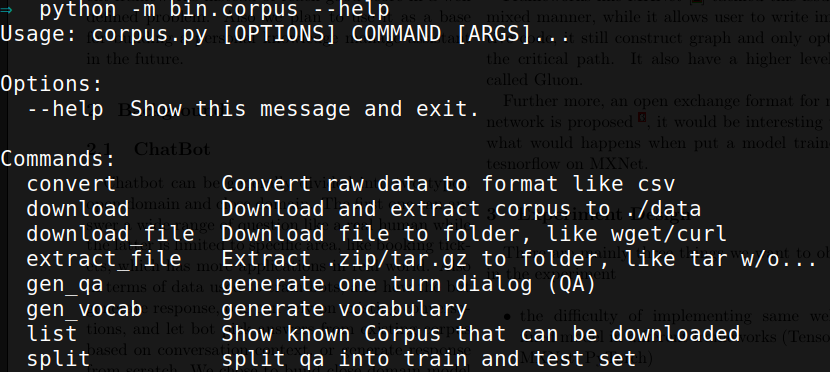
\includegraphics[width=\columnwidth]{data-pipeline}
    \caption{Data Pipeline command line interface}
    \label{fig:data-pipeline}
\end{figure}

\subsection{Text processing}
\label{subsec:text-processing}

In contrast with previous assignments, we removed a lot of text processing when building the chatbot,
just simply split word by space and ignore invalid codec that can crash the program.
For instance, stop words are not removed, because in a normal chat, we are expecting words like \verb+I+, \verb+a+.
Also we find converting words to lower case does not make much difference (see section~\ref{sec:evaluation}) because
they will have similar word vector given enough data and training time.
Special characters are also not removed, so certain dataset can keep their own feature, like emoji is widely used in twitter
(see section~\ref{subsec:twitter}).

However, we added an extra step of removing high frequency general dialogs from corpus like \verb+I don't know+,
which gives use a better result, but the alternatives are still quite general.
Another addition formatting dataset into a standard format of question and answer.
All of the text processing are in our data pipeline tool (see section~\ref{subsec:data-pipeline}) with around 600 lines of python code.

%\subsection{Tensorflow Seq2Seq API}
%\label{subsec:tf-seq2seq}

\subsection{Seq2Seq Frameworks}
\label{subsec:seq2seq-frameworks}

In our experiments we use existing seq2seq frameworks, there are plenty of them, as shown in Table~\ref{table:seq2seq-frameworks}.
We chose OpenNMT-tf and sockeye because we are interested in the rumor that MXNet is more efficient on using GPU memory than Tensorflow.

\begin{table}[h]
    \caption{Seq2Seq Frameworks}
    \label{table:seq2seq-frameworks}
    \centering
    \begin{tabular}{llll}
        \toprule
        Name & Framework & GitHub & Star \\
        \midrule
        OpenNMT-py & PyTorch & \href{https://github.com/OpenNMT/OpenNMT-py}{OpenNMT/OpenNMT-py} & 773 \\
        OpenNMT & Torch & \href{https://github.com/OpenNMT/OpenNMT}{OpenNMT/OpenNMT} & 1461 \\
        OpenNMT-tf & Tensorflow & \href{https://github.com/OpenNMT/OpenNMT-tf}{OpenNMT/OpenNMT-tf} & 145 \\
        nmt & Tensorflow & \href{https://github.com/tensorflow/nmt}{tensorflow/nmt} & 2094 \\
        seq2seq & Tensorflow & \href{https://github.com/google/seq2seq}{google/seq2seq} & 3019 \\
        tensor2tensor & Tensorflow & \href{https://github.com/tensorflow/tensor2tensor}{tensorflow/tensor2tensor} & 2975 \\
        Sockeye & MXNet & \href{https://github.com/awslabs/sockeye}{awslabs/sockeye} & 290 \\
        \bottomrule
    \end{tabular}
\end{table}

Although most of them are built for neural machine translation, we can use them for chatbot directly by swapping the input
and output file as show in Table~\ref{table:seq2seq-app}.

\subsubsection{Sockeye (MXNet)}
\label{subsubsec:sockeye}

Sockeye only requires two text file, it was expecting two different language, but we replace it with questions and answers in same language.
It will generate the vocabulary on the fly, it simply splits sentence into tokens by space, no conversion like remove special token is performed.
(But we did the pre-processing and joined the processed text with space.) It supports attention and beam search.

\subsubsection{OpenNMT-tf (Tensorflow)}
\label{subsubsec:opennmt-tf}

OpenNMT-tf use a YAML file as config, which is similar across all OpenNMT implementation.
It also supports attention and beam search, but its default configuration is not very practical.
It asks you to set train step instead of epoch, and seems don't support auto stop when there is no more improvement after k epoch.

\section{Evaluation}
\label{sec:evaluation}

We run our experiment on a normal desktop with a NVIDIA GTX 1080 8GB.
We use 2 layer LSTM with 256 hidden units, (took around 5GB RAM and has 66157396 parameters), vocabulary size is 50000 (covers 90\%+).
Attention is used and beam size is set to 5 for beam search (there is no randomness injected, so the response is quite deterministic).
Normally it took 1h (around 7 epoch) for sockeye to reach the best result, it will continue 3 epoch before stop training.
For OpenNMT-tf, the default config would take 83.7h to finish training (1000000 steps), so we force it to stop after 1h.

One thing to note is there is no hard metrics for evaluating a chatbot~\cite{liu2016not}.
We use perplexity like NMT, to represent how close we approach when training.
For Cornell dataset, the best perplexity in training on evaluation set is 90, for Twitter dataset, the best perplexity is 135.
However, the most popular way for testing a dialog system now is to employ human to give judgement (i.e. is this a bot or a human),
which is quite expensive, so we skipped it and only tested it among team members.

\subsection{Word embedding}
\label{subsec:word-embedding}

We didn't initialize our embedding matrix with pre-trained value from word2vec or GloVe, and let they be part of the parameters and trained along.
Although our data is not large, but it's big enough to capture the similarity of words, so even without careful text processing (section ~\ref{subsec:text-processing}),
our eventual result won't suffer much from that,
because words like \verb+love+ and \verb+Love+ does not have very large distance as shown in figure~\ref{fig:embedding-love}
\footnote{you can also use tensorboard for mxnet based application \url{https://github.com/dmlc/tensorboard}}.
We did normalize text in some runs, but since it's hard to evaluate automatically,
we find little difference for the limited input we have tried.

\begin{figure}[h]
    \centering
    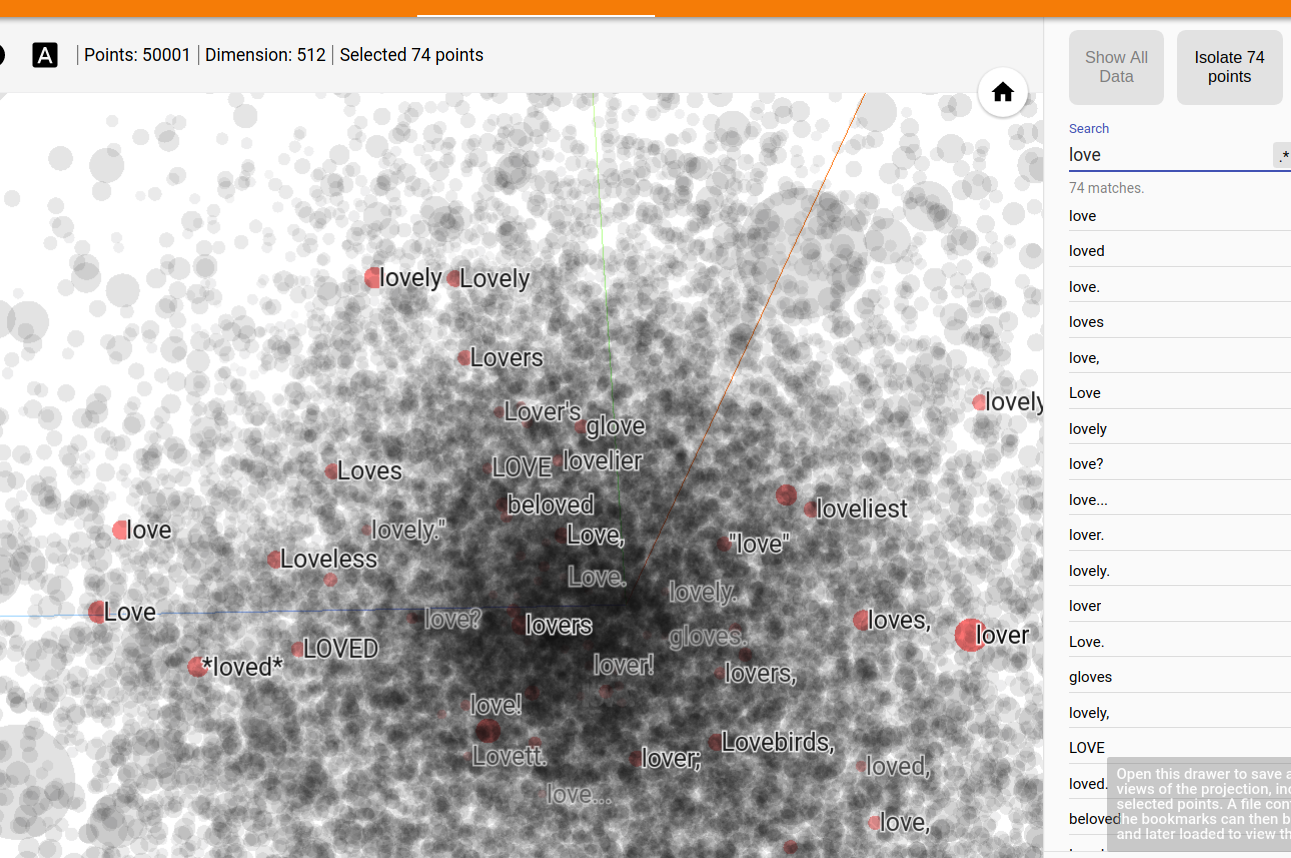
\includegraphics[width=\columnwidth]{embedding-love}
    \caption{Word embedding with random initialization}
    \label{fig:embedding-love}
\end{figure}

\subsection{Entity recognition}
\label{subsec:entity-recognition}

Although we didn't implement named entity recognition (which is a core part of industrial strength chatbot).
Some dialog can shows our naive end to end framework can capture simple entity like refer to different person \verb+he, she, I+
(Table~\ref{table:entity-recognition}).
However the grammar can be very wrong i.e. \verb+I don't what I was+,
it's likely to be caused by \verb+I was+ appers much more than \verb+I am+ in training data.

\begin{table}[h]
    \caption{Simple entity recognition}
    \label{table:entity-recognition}
    \centering
\begin{tabular}{p{65mm}|p{75mm}}
  \toprule
  Cornell Movie Dialog & Twitter Chat \\
  \hline
Q: what do you think about him \newline
A: what do you mean? \newline
Q: where is he \newline
A: i don't know what he is. \newline
Q: where is she \newline
A: she said she was a <unk> \newline
Q: she said what? \newline
A: she said she was a <unk> \newline
Q: he said what? \newline
A: he said he was a <unk> \newline
Q: i said what? \newline
A: what do you want?
  &
Q: where is he \newline
A: i think he is a <unk> \newline
Q: where is she \newline
A: i don't know what she was in the <unk> \newline
Q: where is him \newline
A: i think he is a <unk> \newline
Q: where is her \newline
A: i don't know what she was in the <unk> \newline
Q: where am i \newline
A: i don't know what i was in the <unk> \newline
Q: what is he doing \newline
A: i think he is a <unk> \newline
Q: what is she doing \newline
A: i think she is a <unk> \newline
Q: what am i doing \newline
A: i don't know what you want to do with the <unk>
  \\
  \bottomrule
\end{tabular}
\end{table}

\subsection{Generic Response}
\label{subsec:generic-response}

There are a lot generic responses in the chats we have listed (Table~\ref{table:cornell-idk}, ~\ref{table:cornell-twitter}, ~\ref{table:entity-recognition}).
It's a common problem if look at all the chatbots using seq2seq only.
Attention is said to be able to improve this, but we didn't see much difference when attention is applied.
We believe this can't be solved easily if we stick to a simple end to end framework like seq2seq,
extra knowledge must be introduced, like named entity recognition.
When training data is relative large, the model will fit to the most common dialogs, which falls to \verb+I don't know+,
\verb+what do you mean+.
Some people chose to train the already trained model with very small dataset to generate more vivid dialog,
which we believe is just a more advanced trick of using hard coded rules to shrink the domain of response and is not a general solution.

Also, we believe the generic response also have a lot to do with our dataset.
The Cornell Movie Dialog Corpus we are using is quite dramatic, it's script for movie after all.
It would be better to have corpus that covers people's daily life.
Ubuntu Corpus~\cite{lowe2015ubuntu} might be a good choice, it is very technical but more closer to daily life.
Twitter no longer allows people to scrap and share data, people doing that has legal issues.
There are people sharing Reddit data (1TB) but we haven't tried that yet.


\section{Conclusion}
\label{sec:conclusion}

We built an open domain generative chatbot using seq2seq model with Tensorflow and MXNet respectively.
The bot is able to capture simple entity, but most responses are pretty generic.
End to end model using seq2seq is easy to implement, but using it alone can't yield good result.
In the future we plan to try entity recognition and larger dataset with distributed training,
and might switch to retrieval based chatbot.

The workload in the project is distributed as following

\begin{itemize}
    \item Pinglei Guo: Data Pipeline, Part of Tensorflow of MXNet based implementation
    \item Yusi Xiang: Twitter Data, Part of MXNet based implementation
    \item Yunzheng Zhang: Cornell Data, Part of Tensorflow based implementation
    \item Weiting Zhan: Twitter Data, Test, Report
\end{itemize}

The authors like to thank Tianyi Luo and Haiyu Yang for advice on the seq2seq model and organizing python codebase.

\printbibliography

%\section*{Appendix: A}
%\label{sec:appendix:a}

\end{document}